\documentclass[main]{subfiles}


\title[AutoML: NAS]{Neural Architecture Search}
\subtitle{How to evaluate Neural Architecture Search?}
\author[Jovita Lukasik]{Jovita Lukasik}
\date{}

\titlebackground*{images/AutoML_HPO_2_2}

%\institute{}
%\date{}

\begin{document}
	
	\maketitle


\begin{frame}{Search Strategies}
\begin{center}
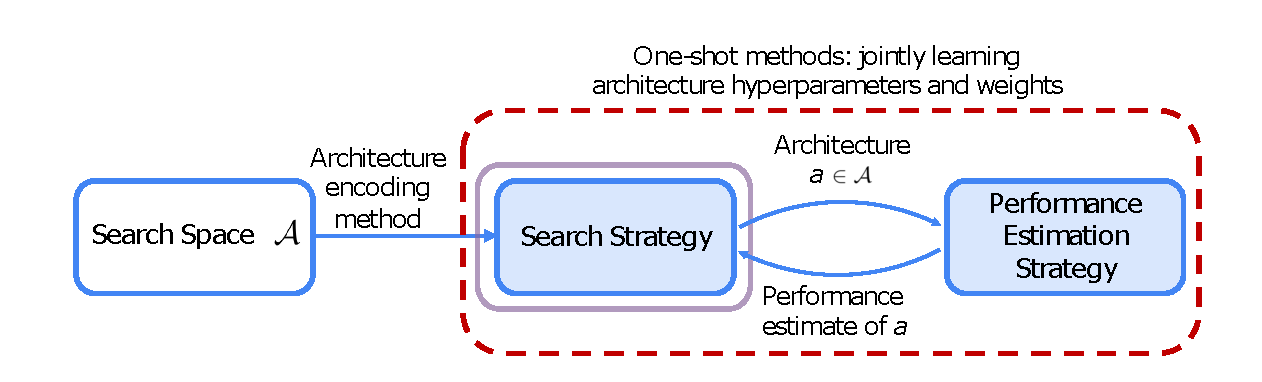
\includegraphics[height=3cm]{images/03/white_2023_nas_overview_2.pdf}
\captionof{figure}{Overview of neural architecture search ~\liturl{White et al. 2023}{https://arxiv.org/pdf/2301.08727.pdf}}
\end{center}
The search strategy aims to find the optimal architecture.
Search strategies can be split in two different categories:
\begin{itemize}
    \item Black-box optimization techniques
    \item One-shot techniques
\end{itemize}
    
\end{frame}

\begin{frame}{Black-Box Optimization Techniques}
\begin{itemize}
    \item Basic algorithms
        \begin{itemize}
            \item Random search
            \item Local search
        \end{itemize}
    \item Bayesian optimization 
    \item Evolution algorithm
\end{itemize}
Black-box optimization techniques are widels used due to strong performance
Tend to use more computational resources than one-shot techniques
\end{frame}

\begin{frame}{Basic Algorithms}
Random search:
\begin{itemize}
    \item Select architectures randomly from search space and fully trains them
    \item Architecture with the best score is the output
\end{itemize}
    $\rightsquigarrow$ Strong baseline

Pros:
\begin{itemize}
    \item Performs well on highly engineered search spaces with a high amount of high scoring architectures
\end{itemize}
Cons:
\begin{itemize}
    \item Not the best performance on large, diverse search spaces
\end{itemize}
\end{frame}

\begin{frame}{Basic Algorithms}
Local search:
\begin{itemize}
    \item Iteratively trains and evaluate all neighbors of the best architecture found so far
    \item Neighborhood: All architectures that differ by one operation or edge
\end{itemize}
$\rightsquigarrow$  Strong baseline of small and large search spaces
\end{frame}

\begin{frame}{Evolutionary and Genetic Algorithms}
Evolutionary algorithm:
\begin{itemize}
    \item Iteratively updating a population of architectures
    \item In each step one (or more) parent architecture (mostly high scoring architecture) in population sampled, combined and mutated to create new children architectures
    \item Children are trained and added to population and replace individuals (with worse scores)
\end{itemize}
\end{frame}

\begin{frame}{Evolutionary and Genetic Algorithms}
Methods differ in several steps:
\begin{itemize}
    \item Initial population sampling 
    \begin{enumerate}
        \item Using trivial architectures
        \item Random sampling
        \item Hand-picked high scoring architectures
    \end{enumerate}
    \item Parents selection (is core component)
    \begin{enumerate}
        \item Tournament selection, i.e., selecting best architecture(s) out of random population
        \item Random sampling weighted by fitness
        \item Choosing current best architecture(s) as parents 
        \item Trade off exploration vs exploitation the best region found so far
    \end{enumerate}
    \item Children generation 
\end{itemize}
\end{frame}

\begin{frame}{Regularized Evolution}
Regularized evolution~\liturl{Real et al. 2019}{https://www.google.com/url?sa=t&source=web&rct=j&opi=89978449&url=https://ojs.aaai.org/index.php/AAAI/article/view/4405/4283&ved=2ahUKEwjzwIKVnqiFAxVEWEEAHRuOBKgQFnoECBUQAQ&usg=AOvVaw2qydwc3_uYx8OTuo5S7RYV} is the most successful evolutionary algorithm method
\begin{itemize}
    \item Search for blocks (cells) with 5 choices (applied on the NASNet search space~\liturl{Zoph et al. 2018}{https://openaccess.thecvf.com/content_cvpr_2018/papers/Zoph_Learning_Transferable_Architectures_CVPR_2018_paper.pdf}):
    \begin{itemize}
        \item Choose 2 previous feature maps
        \item Choose operations for both (convolutions, pooling)
        \item Choose operation to merge (add or concat)
    \end{itemize}
    \item Evolution simply tackles this as a \textit{hyperparameter optimization}(HPO) problem with $2 \times 5$ variables
    \item Worst/oldest solution is dropped from the population
\end{itemize}
    \alert{Novelty:} Dropping the architecture in each step, which has been in the population the longest (even if its the best)
    Achieved state-of-the-art performance on ImageNet~\liturl{Deng et al. 2009}{https://ieeexplore.ieee.org/stamp/stamp.jsp?tp=&arnumber=5206848} at release time
\end{frame}

\begin{frame}{Bayesian Optimization for NAS}
Bayesian optimization (BO) is a powerful tool for optimizing expensive functions
\begin{itemize}
    \item Two key components
    \begin{enumerate}
        \item Probabilistic surrogate
        \item Acquisition function
    \end{enumerate}
    \item Iterative algorithm
    \begin{enumerate}
        \item Selecting architecture maximizing the acquisition function (computing  using the surrogate)
        \item Training the architecture
        \item Retraining the surrogate
    \end{enumerate}
\end{itemize}
\end{frame}

\begin{frame}{Bayesian Optimization for NAS}
Initial Bayesian optimization approaches for NAS:
\begin{itemize}
    \item Custom distance metric (NASBOT)
    \item Gaussian process surrogate with BO
    \item Tree-Parsen estimator
    \item Random forest
    \item Neural Network
    \item Latent space-based BO
    \item Graph-based kernel
\end{itemize}
\end{frame}

\begin{frame}{Bayesian Optimization for NAS}
Acquisition functions popular in NAS:
\begin{itemize}
    \item Expected improvement
    \item Upper confidence bound
\end{itemize}
\end{frame}

\begin{frame}{Bayesian Optimization for NAS}
\begin{itemize}
    \item Encode architecture space by categorical hyperparameters 
    \item Strong performance with tree-based methods:
    \begin{itemize}
        \item TPE: Joint optimization of a vision architecture with 238 hyperparameters ~\liturl{Bergstra et al. 2013}{https://proceedings.mlr.press/v28/bergstra13.pdf}
        \item SMAC~\liturl{Hutter et al. 2011}{https://www.google.com/url?sa=t&source=web&rct=j&opi=89978449&url=https://ml.informatik.uni-freiburg.de/wp-content/uploads/papers/11-LION5-SMAC.pdf&ved=2ahUKEwjhvq__oaiFAxWfQEEAHQ9LAMUQFnoECBEQAQ&usg=AOvVaw0JDLCAOFREpqWduCjgVrzM} Joint architecture and hyperparameter search\\ $\rightarrow$ Auto-Net~\liturl{Mendoza et al. 2016}{http://proceedings.mlr.press/v64/mendoza_towards_2016.pdf}
    \end{itemize}
    \item Kernels for Gaussian processes- based NAS	
    \begin{itemize}
        \item NASBOT~\liturl{Kandasamy et al. 2018}{https://proceedings.neurips.cc/paper_files/paper/2018/file/f33ba15effa5c10e873bf3842afb46a6-Paper.pdf}
    \end{itemize}
    \item BO approaches using neural networks 
     \begin{itemize}
        \item  BANANAS~\liturl{White et al. 2021}{https://www.google.com/url?sa=t&source=web&rct=j&opi=89978449&url=https://ojs.aaai.org/index.php/AAAI/article/view/17233/17040&ved=2ahUKEwjb-tPvoqiFAxVEZ0EAHbjrD2AQFnoECBAQAQ&usg=AOvVaw2TJIMtnKMZjY0mC-YmStCO}
    \end{itemize}
    \item BO very competitive, has been shown to outperform RL \liturl{Ying et al. 2019}{https://proceedings.mlr.press/v97/ying19a/ying19a.pdf}
\end{itemize}
\end{frame}

\begin{frame}{Black-Box Optimization Technqiues}
Pros:
\begin{itemize}
    \item Widely used due to strong performance
    \item More robust 
    \item Simpler optimization
    \item Joint optimization with other hyperparameters
    \item Allows for easier adaptation to new problems, datasets, search spaces
    \item Often conceptually simpler
\end{itemize}
Cons:
\begin{itemize}
    \item Tend to use more computational resources than one-shot techniques
\end{itemize}
\end{frame}
%----------------------------------------------------------------------
\begin{frame}{Summary} 

Most important insights from this video:

\begin{enumerate}
    \item ???
    \item ???
    \item ???
\end{enumerate}


\end{frame}



\end{document}
